% =====================================================================
% Modelo para Relatório Final de Iniciação Científica (em Português)
% Prof. Vítor E. Silva Souza - NEMO / PPGI / DI / UFES
%
% Baseado no modelo fornecido pela PRPPG/UFES:
% https://prppg.ufes.br/programa-institucional-de-ic-piic
%
% O modelo já preenche grande área e área CNPq para a Computação.
% Procurar por textos envolvidos em \hl{}, ler as instruções e 
% substituir pelo texto do relatório.
% =====================================================================
\documentclass[10pt, a4paper]{article}

% Seleção de códigos de fonte.
\usepackage[T1]{fontenc}

% Codificação do documento em Unicode.
\usepackage[utf8]{inputenc}

% Especifica o uso de português do Brasil.
\usepackage[portuges,brazilian]{babel}

% Controle das cores.
\usepackage[usenames,dvipsnames]{xcolor}

% Inclusão de gráficos.
\usepackage{graphicx}

% Posicionamento de elementos.
\usepackage{float}

% Melhor controle de layout em tabelas.
\usepackage{tabularx}

% Permite usar tabelas que ocupam mais de uma página
\usepackage{longtable}
\usepackage{colortbl}

% \rm is deprecated and should not be used in a LaTeX2e document
% http://tex.stackexchange.com/questions/151897/always-textrm-never-rm-a-counterexample
\renewcommand{\rm}{\textrm}

% Inclusão de símbolos não padrão.
\usepackage{amssymb}
\usepackage{eurosym}

% Para utilizar \eqref para referenciar equações.
\usepackage{amsmath}

% Permite mostrar figuras muito largas em modo paisagem com \begin{sidewaysfigure} ao invés de \begin{figure}.
\usepackage{rotating}

% Permite customizar listas enumeradas/com marcadores.
\usepackage{enumitem}

% Permite inserir hiperlinks com \url{}.
\usepackage{bigfoot}
\usepackage[hidelinks]{hyperref}

% Permite usar o comando \hl{} para evidenciar texto com fundo amarelo. Útil para chamar atenção a itens a fazer.
\usepackage{soulutf8}

% Permite inserir espaço em branco condicional (incluído no texto final só se necessário) em macros.
\usepackage{xspace}

% Permite inserir comentários para controle de revisão de documentos.
\usepackage[colorinlistoftodos, textwidth=20mm, textsize=footnotesize]{todonotes}
\newcommand{\aluno}[1]{\todo[author=\textbf{Aluno},color=green!30,caption={},inline]{#1}}
\newcommand{\vitor}[1]{\todo[author=\textbf{Vítor},color=red!30,caption={},inline]{#1}}

% Permite incluir listagens de código com o comando \lstinputlisting{}.
\usepackage{listings}
\usepackage{caption}
\DeclareCaptionFont{white}{\color{white}}
\DeclareCaptionFormat{listing}{\colorbox{gray}{\parbox{\textwidth}{#1#2#3}}}
\captionsetup[lstlisting]{format=listing,labelfont=white,textfont=white}
\renewcommand{\lstlistingname}{Listagem}
\definecolor{mygray}{rgb}{0.5,0.5,0.5}
\lstset{
	basicstyle=\scriptsize,
	breaklines=true,
	numbers=left,
	numbersep=5pt,
	numberstyle=\tiny\color{mygray}, 
	rulecolor=\color{black},
	showstringspaces=false,
	tabsize=2,
	inputencoding=utf8,
	extendedchars=true,
	literate=%
	{é}{{\'{e}}}1
	{è}{{\`{e}}}1
	{ê}{{\^{e}}}1
	{ë}{{\¨{e}}}1
	{É}{{\'{E}}}1
	{Ê}{{\^{E}}}1
	{û}{{\^{u}}}1
	{ù}{{\`{u}}}1
	{â}{{\^{a}}}1
	{à}{{\`{a}}}1
	{á}{{\'{a}}}1
	{ã}{{\~{a}}}1
	{Á}{{\'{A}}}1
	{Â}{{\^{A}}}1
	{Ã}{{\~{A}}}1
	{ç}{{\c{c}}}1
	{Ç}{{\c{C}}}1
	{õ}{{\~{o}}}1
	{ó}{{\'{o}}}1
	{ô}{{\^{o}}}1
	{Õ}{{\~{O}}}1
	{Ó}{{\'{O}}}1
	{Ô}{{\^{O}}}1
	{î}{{\^{i}}}1
	{Î}{{\^{I}}}1
	{í}{{\'{i}}}1
	{Í}{{\~{Í}}}1
}

% Configurações de bibliografia.
\usepackage{natbib}
\let\oldbibliography\thebibliography
\renewcommand{\thebibliography}[1]{\oldbibliography{#1}\setlength{\itemsep}{0pt}}

% Redefinição das fontes usadas no documento.
\usepackage{helvet}
\renewcommand{\familydefault}{\sfdefault}

% Define margens e espaçamentos personalizados para o documento.
\usepackage{anysize}
\marginsize{30mm}{30mm}{15mm}{15mm}
\setlength{\headsep}{1.5cm}
\renewcommand{\baselinestretch}{1.5}

% Pacotes incluídos no modelo da PRPPG e não utilizados:
%\usepackage{ifthen}
%\usepackage{array}
%\usepackage{enumerate}
%\usepackage{adjustbox}
%\usepackage{caption}
%\usepackage{subcaption}
%\usepackage{mathptmx}

% Cabeçalho.
\usepackage{fancyhdr}
\usepackage{afterpage}
\pagestyle{fancy}
\fancyhf{} % clear all fields
\fancyhead[R]{Universidade Federal do Espírito Santo\\ Programa Institucional de Iniciação Científica\\
	Relatório Final de Pesquisa\\
	Ciências Exatas e da Terra}
\renewcommand{\headrulewidth}{0pt}

% Orientações:
% Este documento deve ser utilizado como modelo para a elaboração do Relatório Final dos Subprojetos do programa Institucional de Iniciação Científica da UFES. Deve-se utilizar na elaboração do relatório alinhamento justificado e fonte Times New Roman, corpo 10 com espaçamento entre linhas de 1,5, e tamanho 12 para títulos.
%
% LEMBRE-SE: O RELATÓRIO FINAL É INDIVIDUAL E DEVE SER ESCRITO PELO BOLSISTA/VOLUNTÁRIO DE INICIAÇÃO CIENTÍFICA, SOB A SUPERVISÃO DO SEU ORIENTADOR. O RELATÓRIO DEVERÁ SER ENVIADO PELO ORIENTADOR ATRAVÉS DO SISTEMA DO PROGRAMA INSTITUCIONAL DE INICIAÇÃO CIENTÍFICA (PIIC) ATÉ A DATA LIMITE DE ESTABELECIDA NO EDITAL. O LINK PARA ENVIO DO RELATÓRIO ESTÁ DISPONÍVEL NO SISTEMA DO PIIC A PARTIR DO DIA DE INÍCIO DE ENVIO ESTABELECIDO NO EDITAL.
%
% O ENVIO DO RELATÓRIO FINAL APÓS A DATA LIMITE ESTABELECIDA IMPLICARÁ NO IMPEDIMENTO DE PARTICIPAÇÃO DO ORIENTADOR DO(S) E DOS BOLSISTA(S) OU VOLUNTÁRIO(S) EM FUTURAS EDIÇÕES DO PIIC, CONFORME PREVISTO NO INCISO V DO ITEM 11º DO REGULAMENTO GERAL DO PIIC, DISPONÍVEL NO SITE DA PRPPG.


% Início do documento.
\begin{document}

% "Capa":
\afterpage{\cfoot{\thepage}}
\ 
\vspace{1cm}

\begin{center}
	{\Large \bf \hl{Título do Subprojeto}}
\end{center}

\vspace{.5cm}

{\bf Identificação:}
\begin{tabular}{c l l}
	\phantom{cosmologia}&{Grande área do CNPq:} & Ciências Exatas e da Terra \\
	&{Área do CNPq:} &  Ciência da Computação \\
	&{Título do Projeto:} & \hl{Título do Projeto} \\
	&{Professor Orientador:} & \hl{Orientador} \\
	&{Estudante PIBIC/PIVIC:} & \hl{Nome do Estudante} 
\end{tabular}
\vspace{.5cm}

\begin{quote}
	{\bf Resumo:}
	\emph{\hl{Antes do corpo do texto, deve ser incluído o resumo do trabalho, que deve conter uma breve descrição do subprojeto com seus objetivos e justificativas, metodologia e resultados obtidos. O resumo deve conter no máximo 200 palavras, em itálico.}}
	
	{\bf Palavras chaves:} \hl{Devem fornecer ao leitor uma ideia dos principais temas de interesse de que trata a pesquisa.}
\end{quote}

	
	
%%% Início de seção. %%%
\section{Introdução}
\label{sec-intro}

\hl{Ler instruções abaixo e substituir pelo texto do seu relatório.}

O Relatório Final de Iniciação Científica deverá ser enviado pelo orientador através da intranet da PRPPG (http://portais.ufes.br/posgrad/), utilizando o link “Iniciação Científica” disponível no menu “pesquisa/projetos”. O restante deste documento apresenta instruções de conteúdo e formatação para a elaboração do Relatório Final.

O texto deve ser preparado de acordo com as seguintes instruções: (i) o documento não deve exceder 15 páginas de formato A4 com margens de 3 cm (em todos os lados), usando fonte Times New Roman, corpo 10 com espaçamento entre linhas de 1,5 e tabulação de 1 cm no início de cada parágrafo, (ii) as citações e referências bibliográficas devem seguir o formato da ABNT, (iii) a seção de referências bibliográficas deve conter apenas artigos citados no texto, ou seja, “não liste se não citar” e “não cite se não listar”, (iv) os títulos das seções e seus conteúdos devem seguir as recomendações descritas no corpo do texto deste modelo, (v) o cabeçalho das páginas deve ser mantido de acordo com a formatação deste modelo (Times New Roman, corpo 9, alinhado à direita), sendo que a quarta linha do cabeçalho deve ser alterada para descrever a Grande Área de Conhecimento do projeto, isto é, Ciências Exatas e da Terra, Ciências Biológicas, Engenharias, Ciências da Saúde, Ciências Agrárias, Ciências Sociais Aplicadas, Ciências Humanas ou Lingüística, Letras e Artes.

Na introdução, o autor deve apresentar uma descrição geral do tema de estudo, mostrando a relevância do tema estudado, citando, sempre que possível, trabalhos de outros autores para permitir a contextualização de sua pesquisa. O autor também deverá delimitar claramente seu subprojeto dentro do projeto de pesquisa de seu orientador. 

Exemplo de referência bibliográfica: \cite{guarino-et-al:hobook09} (in-line) ou \citep{guarino-et-al:hobook09}.



%%% Início de seção. %%%
\section{Objetivos}
\label{sec-objetivos}

\hl{Descreva de maneira simples e clara os objetivos do subprojeto.}



%%% Início de seção. %%%
\section{Metodologia}
\label{sec-metodo}

\hl{Definir, com base na revisão bibliográfica ou em trabalhos preliminares, a metodologia que deverá ser utilizada para testar a hipótese formulada e atingir os objetivos estabelecidos. Apresentar o procedimento de trabalho, o material que deverá ser utilizado, o tratamento da informação e o procedimento estatístico, se for o caso.}



%%% Início de seção. %%%
\section{Resultados}
\label{sec-resultados}

\hl{Ler instruções abaixo e substituir pelo texto do seu relatório.}

Descreva aqui os resultados ou respostas encontrados durante o trabalho, apresentando os dados/informações obtidos(as) ou coletados(as) e incluindo ilustrações, figuras, fotos ou esquemas. Ilustrações, tabelas ou figuras devem ser numeradas sequencialmente, de acordo com os esquemas de formatação e legendas indicados na Tabela~\ref{tbl-resultadosl-exemplo} e Figura~\ref{fig-resultados-exemplo}. Cada legenda deve ser informativa, com texto alinhado à esquerda, descrevendo o que é mostrado.

\begin{table}
	\caption{Exemplo de formatação de uma tabela para a apresentação de resultados.}
	\label{tbl-resultadosl-exemplo}
	\centering
	\begin{tabular}{ccc}
		\hline
		Grupos de idade [meses] & Número de indivíduos no grupo & Indivíduos viáveis [\%] \\
		\hline
		0--10 & 20 & 9,0 \\
		10--15 & 20 & 10,0 \\
		15--20 & 25 & 4,0 \\
		Acima de 20 & 15 & 3,4  \\
		\hline
	\end{tabular}
\end{table}

\begin{figure}[H]
	\centering
	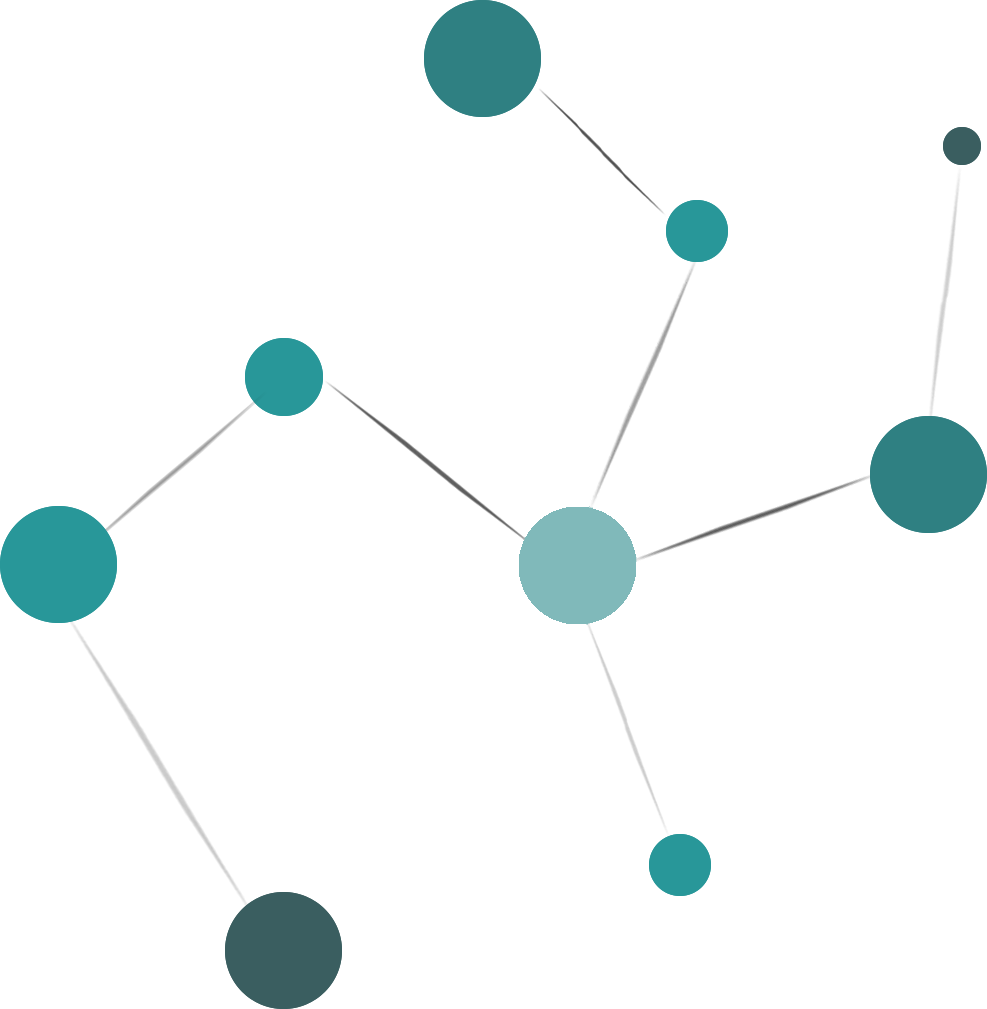
\includegraphics[width=.25\textwidth]{figuras/fig-resultados-exemplo.png} 
	\caption{Exemplo de figura.}
	\label{fig-resultados-exemplo}
\end{figure}

Adicionalmente, a Tabela~\ref{tbl-resultadosl-exemplo-longa} demonstra um exemplo de tabela longa (vide código \LaTeX).

% Tabela longa.
\begin{longtable}{|p{3cm}|p{12cm}|}
	\caption{Exemplo de tabela longa (pode passar de uma página a outra).}
	\label{tbl-resultadosl-exemplo-longa} \\\hline 
	
	% Cabeçalho e repetição do mesmo em cada nova página. Manter como está.
	\rowcolor{lightgray}
	\textbf{Nome} & \textbf{Descrição} \\\hline		
	\endfirsthead
	\hline
	\rowcolor{lightgray}
	\textbf{Nome} & \textbf{Descrição} \\\hline		
	\endhead
	
	% Linhas da tabela.
	Exemplo 01 & Descrição do exemplo 01. \\\hline
	
	Exemplo 02 & Descrição do exemplo 02. \\\hline
	
	Exemplo 03 & Descrição do exemplo 03. \\\hline
\end{longtable}



%%% Início de seção. %%%
\section{Discussão e Conclusões}
\label{sec-conclusoes}

\hl{Ler instruções abaixo e substituir pelo texto do seu relatório.}

A apresentação dos resultados obtidos deve ser seguida de uma seção contendo a discussão sobre o significado dos resultados obtidos. Preferencialmente, as discussões devem contemplar os seguintes aspectos: 

\begin{itemize}	
	\item O que estas respostas ou dados obtidos significam? 
	\item Como elas ajudam a resolver o problema? 
	\item Descrição dos dados à luz da literatura, isto é, como as respostas obtidas se comparam com os dados de literatura.
	\item Quais as possíveis fontes de erro e seu efeito sobre os dados ou análises?
	\item Quais as principais dificuldades encontradas? 
	\item Quais as perspectivas de continuidade do trabalho?
	\item Se seus experimentos ou análises falharam, quais as sugestões para corrigir o problema?	
\end{itemize}

Opcionalmente, conforme as especificidades de cada área do conhecimento, o autor pode utilizar a Seção~\ref{resultados} para apresentação de resultados e sua discussão, deixando a Seção~\ref{conclui} apenas para as conclusões. Neste caso, o título da Seção~\ref{resultados} deverá ser “Resultados e Discussões” e da Seção~\ref{conclui} será “Conclusões”, que deve apresentar um breve resumo dos resultados (ou respostas) mais significativos obtidos, fazendo uma análise crítica do trabalho e descrevendo as perspectivas de continuidade do trabalho.


% Bibliografia.
\bibliographystyle{hapalike2-NOand}
\bibliography{bibliografia}

% Fim do documento.
\end{document}



